% Options for packages loaded elsewhere
% Options for packages loaded elsewhere
\PassOptionsToPackage{unicode}{hyperref}
\PassOptionsToPackage{hyphens}{url}
\PassOptionsToPackage{dvipsnames,svgnames,x11names}{xcolor}
%
\documentclass[
  spanish,
  letterpaper,
  DIV=11,
  numbers=noendperiod]{scrartcl}
\usepackage{xcolor}
\usepackage{amsmath,amssymb}
\setcounter{secnumdepth}{-\maxdimen} % remove section numbering
\usepackage{iftex}
\ifPDFTeX
  \usepackage[T1]{fontenc}
  \usepackage[utf8]{inputenc}
  \usepackage{textcomp} % provide euro and other symbols
\else % if luatex or xetex
  \usepackage{unicode-math} % this also loads fontspec
  \defaultfontfeatures{Scale=MatchLowercase}
  \defaultfontfeatures[\rmfamily]{Ligatures=TeX,Scale=1}
\fi
\usepackage{lmodern}
\ifPDFTeX\else
  % xetex/luatex font selection
\fi
% Use upquote if available, for straight quotes in verbatim environments
\IfFileExists{upquote.sty}{\usepackage{upquote}}{}
\IfFileExists{microtype.sty}{% use microtype if available
  \usepackage[]{microtype}
  \UseMicrotypeSet[protrusion]{basicmath} % disable protrusion for tt fonts
}{}
\makeatletter
\@ifundefined{KOMAClassName}{% if non-KOMA class
  \IfFileExists{parskip.sty}{%
    \usepackage{parskip}
  }{% else
    \setlength{\parindent}{0pt}
    \setlength{\parskip}{6pt plus 2pt minus 1pt}}
}{% if KOMA class
  \KOMAoptions{parskip=half}}
\makeatother
% Make \paragraph and \subparagraph free-standing
\makeatletter
\ifx\paragraph\undefined\else
  \let\oldparagraph\paragraph
  \renewcommand{\paragraph}{
    \@ifstar
      \xxxParagraphStar
      \xxxParagraphNoStar
  }
  \newcommand{\xxxParagraphStar}[1]{\oldparagraph*{#1}\mbox{}}
  \newcommand{\xxxParagraphNoStar}[1]{\oldparagraph{#1}\mbox{}}
\fi
\ifx\subparagraph\undefined\else
  \let\oldsubparagraph\subparagraph
  \renewcommand{\subparagraph}{
    \@ifstar
      \xxxSubParagraphStar
      \xxxSubParagraphNoStar
  }
  \newcommand{\xxxSubParagraphStar}[1]{\oldsubparagraph*{#1}\mbox{}}
  \newcommand{\xxxSubParagraphNoStar}[1]{\oldsubparagraph{#1}\mbox{}}
\fi
\makeatother


\usepackage{longtable,booktabs,array}
\usepackage{calc} % for calculating minipage widths
% Correct order of tables after \paragraph or \subparagraph
\usepackage{etoolbox}
\makeatletter
\patchcmd\longtable{\par}{\if@noskipsec\mbox{}\fi\par}{}{}
\makeatother
% Allow footnotes in longtable head/foot
\IfFileExists{footnotehyper.sty}{\usepackage{footnotehyper}}{\usepackage{footnote}}
\makesavenoteenv{longtable}
\usepackage{graphicx}
\makeatletter
\newsavebox\pandoc@box
\newcommand*\pandocbounded[1]{% scales image to fit in text height/width
  \sbox\pandoc@box{#1}%
  \Gscale@div\@tempa{\textheight}{\dimexpr\ht\pandoc@box+\dp\pandoc@box\relax}%
  \Gscale@div\@tempb{\linewidth}{\wd\pandoc@box}%
  \ifdim\@tempb\p@<\@tempa\p@\let\@tempa\@tempb\fi% select the smaller of both
  \ifdim\@tempa\p@<\p@\scalebox{\@tempa}{\usebox\pandoc@box}%
  \else\usebox{\pandoc@box}%
  \fi%
}
% Set default figure placement to htbp
\def\fps@figure{htbp}
\makeatother


% definitions for citeproc citations
\NewDocumentCommand\citeproctext{}{}
\NewDocumentCommand\citeproc{mm}{%
  \begingroup\def\citeproctext{#2}\cite{#1}\endgroup}
\makeatletter
 % allow citations to break across lines
 \let\@cite@ofmt\@firstofone
 % avoid brackets around text for \cite:
 \def\@biblabel#1{}
 \def\@cite#1#2{{#1\if@tempswa , #2\fi}}
\makeatother
\newlength{\cslhangindent}
\setlength{\cslhangindent}{1.5em}
\newlength{\csllabelwidth}
\setlength{\csllabelwidth}{3em}
\newenvironment{CSLReferences}[2] % #1 hanging-indent, #2 entry-spacing
 {\begin{list}{}{%
  \setlength{\itemindent}{0pt}
  \setlength{\leftmargin}{0pt}
  \setlength{\parsep}{0pt}
  % turn on hanging indent if param 1 is 1
  \ifodd #1
   \setlength{\leftmargin}{\cslhangindent}
   \setlength{\itemindent}{-1\cslhangindent}
  \fi
  % set entry spacing
  \setlength{\itemsep}{#2\baselineskip}}}
 {\end{list}}
\usepackage{calc}
\newcommand{\CSLBlock}[1]{\hfill\break\parbox[t]{\linewidth}{\strut\ignorespaces#1\strut}}
\newcommand{\CSLLeftMargin}[1]{\parbox[t]{\csllabelwidth}{\strut#1\strut}}
\newcommand{\CSLRightInline}[1]{\parbox[t]{\linewidth - \csllabelwidth}{\strut#1\strut}}
\newcommand{\CSLIndent}[1]{\hspace{\cslhangindent}#1}

\ifLuaTeX
\usepackage[bidi=basic]{babel}
\else
\usepackage[bidi=default]{babel}
\fi
% get rid of language-specific shorthands (see #6817):
\let\LanguageShortHands\languageshorthands
\def\languageshorthands#1{}


\setlength{\emergencystretch}{3em} % prevent overfull lines

\providecommand{\tightlist}{%
  \setlength{\itemsep}{0pt}\setlength{\parskip}{0pt}}



 


\KOMAoption{captions}{tableheading}
\makeatletter
\@ifpackageloaded{caption}{}{\usepackage{caption}}
\AtBeginDocument{%
\ifdefined\contentsname
  \renewcommand*\contentsname{Tabla de contenidos}
\else
  \newcommand\contentsname{Tabla de contenidos}
\fi
\ifdefined\listfigurename
  \renewcommand*\listfigurename{Listado de Figuras}
\else
  \newcommand\listfigurename{Listado de Figuras}
\fi
\ifdefined\listtablename
  \renewcommand*\listtablename{Listado de Tablas}
\else
  \newcommand\listtablename{Listado de Tablas}
\fi
\ifdefined\figurename
  \renewcommand*\figurename{Figura}
\else
  \newcommand\figurename{Figura}
\fi
\ifdefined\tablename
  \renewcommand*\tablename{Tabla}
\else
  \newcommand\tablename{Tabla}
\fi
}
\@ifpackageloaded{float}{}{\usepackage{float}}
\floatstyle{ruled}
\@ifundefined{c@chapter}{\newfloat{codelisting}{h}{lop}}{\newfloat{codelisting}{h}{lop}[chapter]}
\floatname{codelisting}{Listado}
\newcommand*\listoflistings{\listof{codelisting}{Listado de Listados}}
\makeatother
\makeatletter
\makeatother
\makeatletter
\@ifpackageloaded{caption}{}{\usepackage{caption}}
\@ifpackageloaded{subcaption}{}{\usepackage{subcaption}}
\makeatother
\usepackage{bookmark}
\IfFileExists{xurl.sty}{\usepackage{xurl}}{} % add URL line breaks if available
\urlstyle{same}
\hypersetup{
  pdftitle={Guía de redacción: resultados del TVP--VAR y proxy dinámica de credibilidad},
  pdflang={es},
  colorlinks=true,
  linkcolor={blue},
  filecolor={Maroon},
  citecolor={Blue},
  urlcolor={Blue},
  pdfcreator={LaTeX via pandoc}}


\title{Guía de redacción: resultados del TVP--VAR y proxy dinámica de
credibilidad}
\author{}
\date{}
\begin{document}
\maketitle


::: \{.cell-output .cell-output-stdout\}

\begin{verbatim}
null device 
          1 
\end{verbatim}

:::

\section{Resultados del modelo TVP--VAR y evolución de la credibilidad
monetaria}\label{resultados-del-modelo-tvpvar-y-evoluciuxf3n-de-la-credibilidad-monetaria}

En el apartado anterior, se asumió que existian cambios discretos Las
regresiones móviles presentadas anteriormente sugieren que la
sensibilidad de las expectativas de inflación a 24 meses frente a la
inflación observada no ha permanecido constante durante el período de
estudio. Sobre esa evidencia preliminar, esta sección profundiza el
análisis mediante el TVP--VAR restringido descrito en la metodología. A
diferencia de las estimaciones por ventanas, el modelo permite que la
relación entre inflación y expectativas evolucione de forma continua y,
a partir de ella, recuperar una medida dinámica del desacoplamiento de
las expectativas respecto de la inflación observada, \(\lambda_t\), así
como el nivel del ancla inflacionaria implícita, \(\pi_t^*\). Esta
estrategia mantiene la lógica de Maria Demertzis (2009) y del enfoque de
parámetros variantes utilizado por
(\textbf{strohsal\_melnick\_nautz2015?}), aunque adaptada al horizonte
de expectativas disponible para Guatemala.

\subsection{Evidencia a favor de una relación cambiante entre inflación
y
expectativas}\label{evidencia-a-favor-de-una-relaciuxf3n-cambiante-entre-inflaciuxf3n-y-expectativas}

\begin{longtable}[]{@{}lccc@{}}

\caption{\label{tbl-comparacion-m0-m3}Comparación entre el VAR con
parámetros constantes y el TVP--VAR restringido}

\tabularnewline

\toprule\noalign{}
Modelo & Log-verosimilitud & AIC & BIC \\
\midrule\noalign{}
\endhead
\bottomrule\noalign{}
\endlastfoot
M0 & -184.45 & 384.89 & 411.16 \\
M3 & -146.33 & 312.67 & 345.50 \\

\end{longtable}

La comparación con el VAR de parámetros constantes muestra que permitir
variación temporal en la ecuación de expectativas mejora sustancialmente
el ajuste del sistema. Tanto el AIC como el BIC disminuyen al pasar de
M0 a M3, aun cuando este último incorpora las varianzas de transición
asociadas a \(c_{0t}\) y \(c_t\). En consecuencia, la evidencia de los
criterios de información favorece una representación en la que el
vínculo entre inflación y expectativas puede modificarse gradualmente a
lo largo de la muestra. La razón de verosimilitudes conduce a la misma
dirección, aunque su significancia se interpreta únicamente como
evidencia complementaria debido a que las varianzas de transición se
encuentran en la frontera del espacio paramétrico bajo la hipótesis de
constancia.

El modelo estima varianzas de transición positivas para el intercepto y
para la sensibilidad de las expectativas frente a la inflación, lo que
confirma que ambas dimensiones contienen variación temporal. Asimismo,
el sistema permanece localmente estable durante toda la muestra, pues el
radio espectral se mantiene por debajo de la unidad. Estos resultados
permiten interpretar las trayectorias suavizadas sin evidencia de
dinámica explosiva. Los diagnósticos residuales son satisfactorios para
la ecuación de expectativas y para la correlación contemporánea entre
innovaciones; no obstante, la ecuación de inflación interanual conserva
autocorrelación residual, aspecto que se examina posteriormente mediante
ejercicios de robustez con medidas alternativas de inflación.

\subsection{Evolución de los parámetros variantes de la ecuación de
expectativas}\label{evoluciuxf3n-de-los-paruxe1metros-variantes-de-la-ecuaciuxf3n-de-expectativas}

\begin{figure}

\begin{minipage}{0.50\linewidth}

\centering{

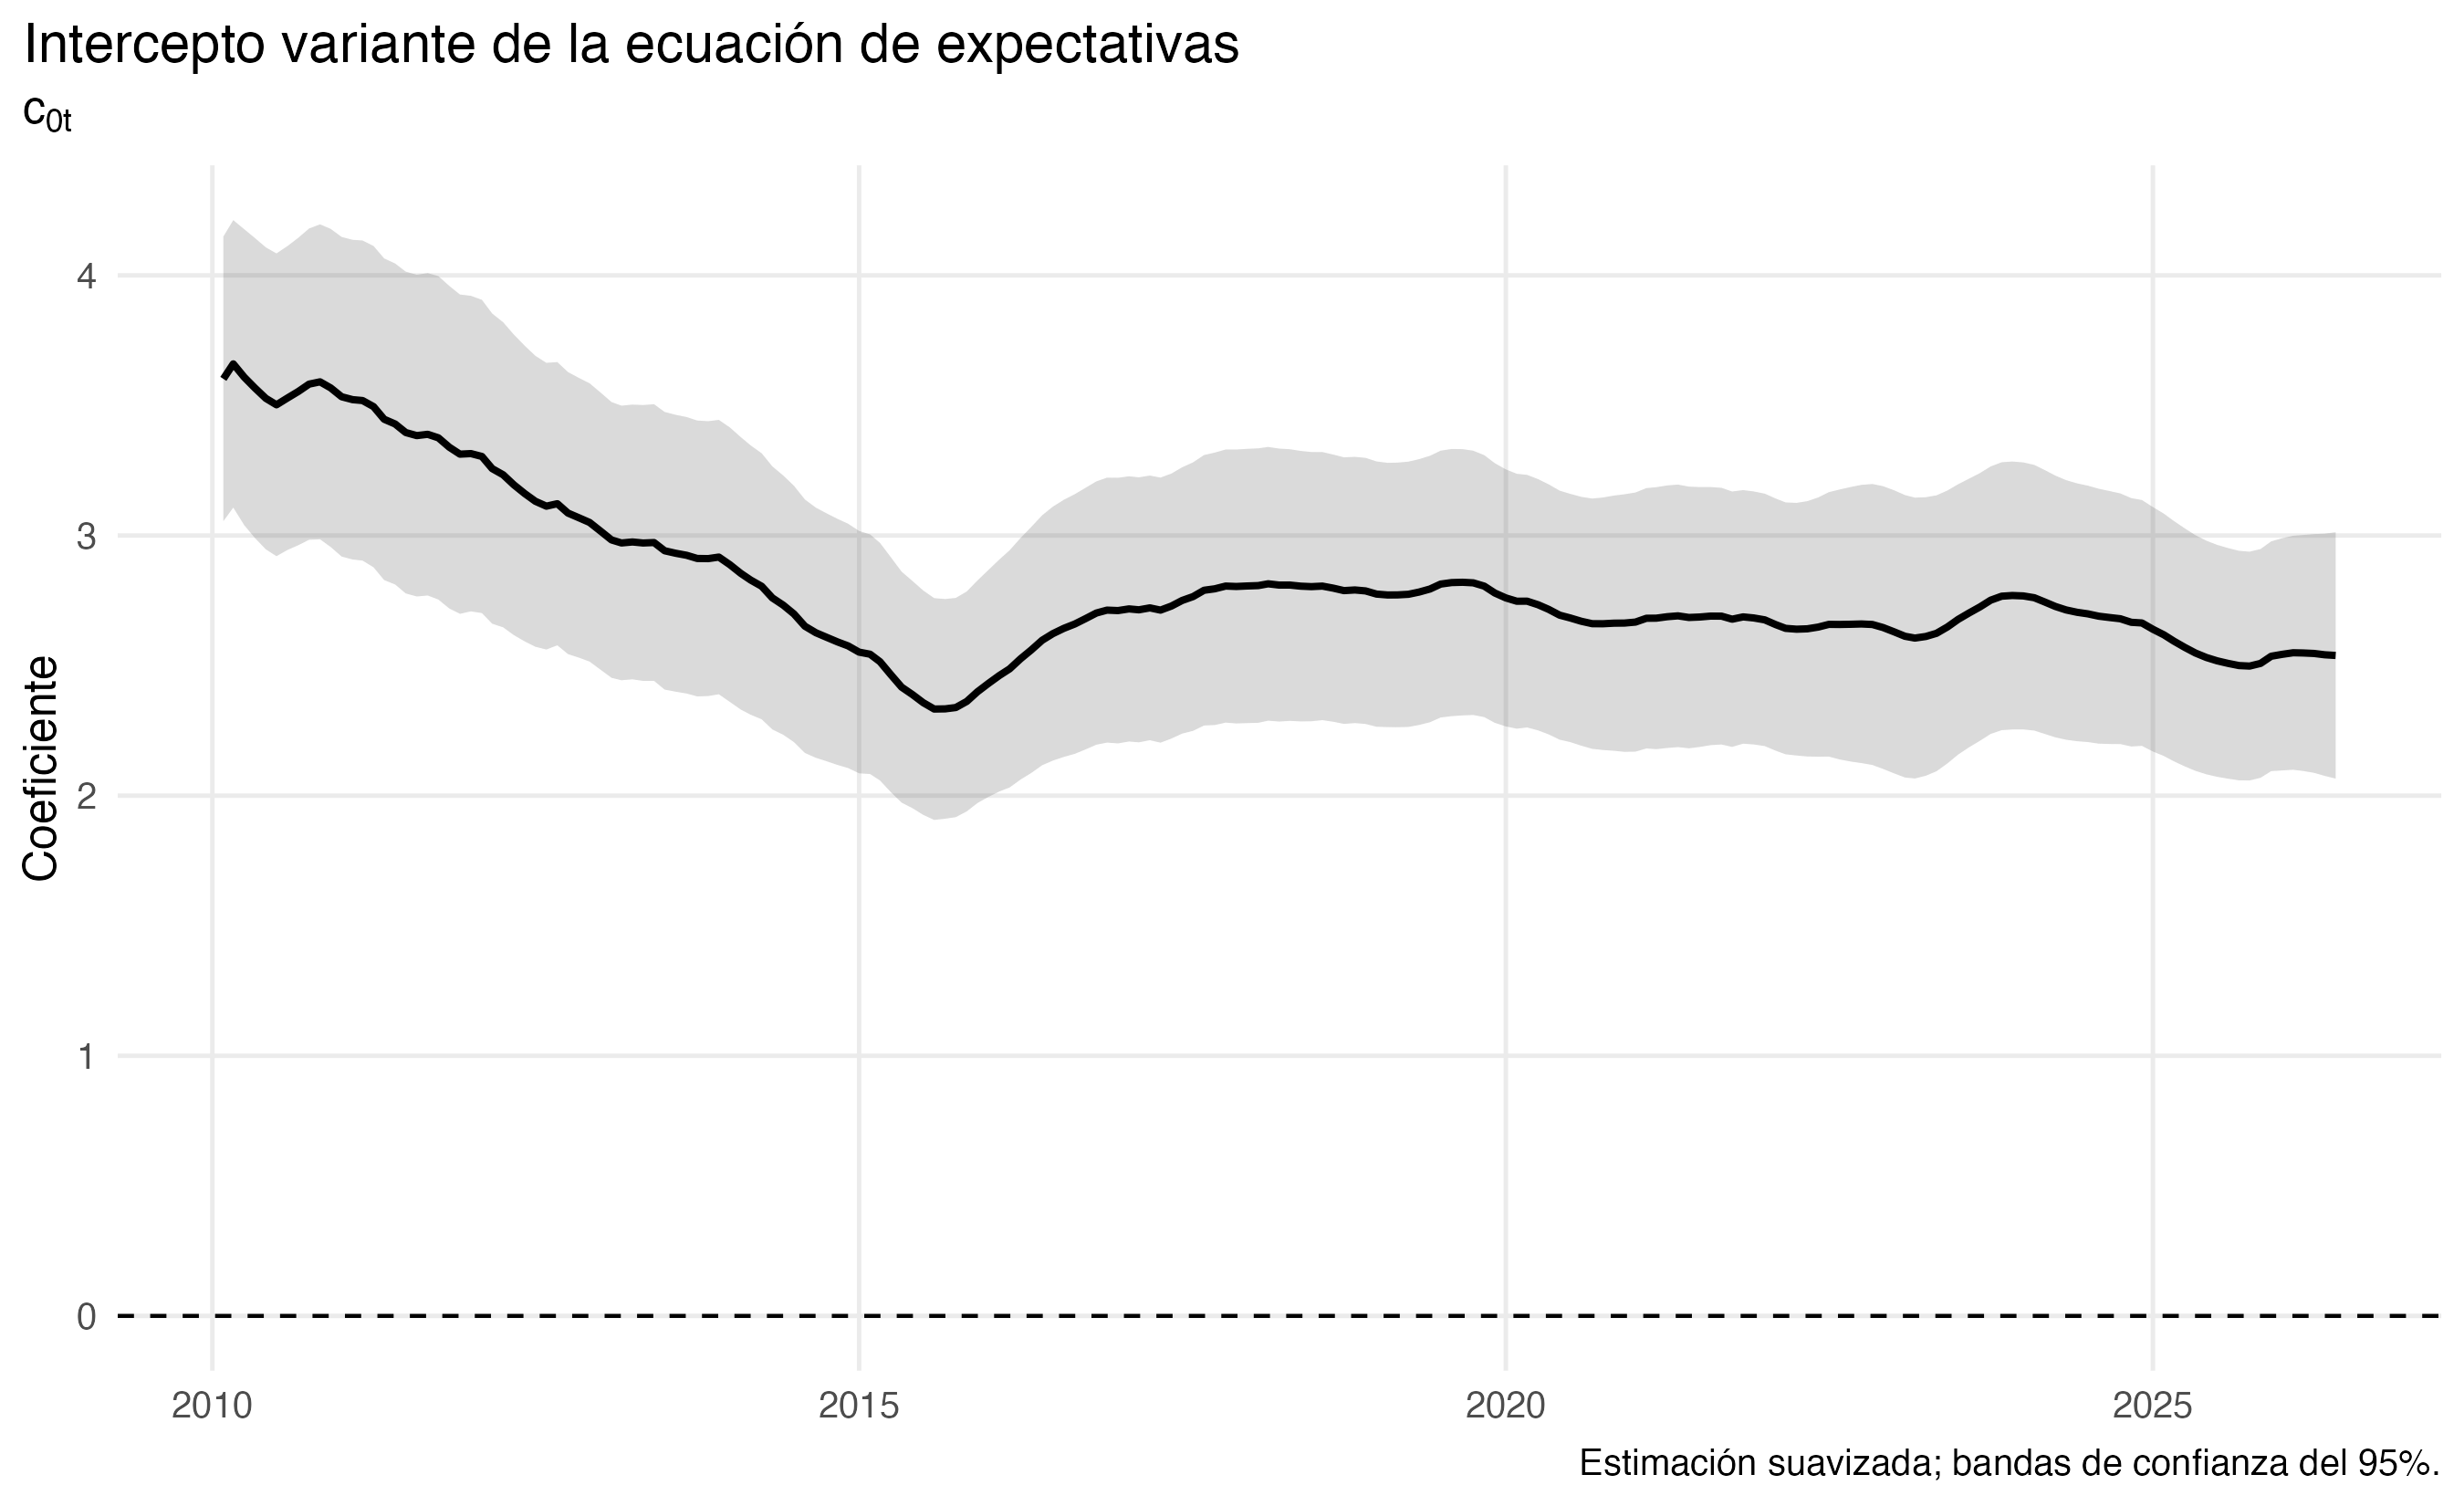
\includegraphics[width=1\linewidth,height=\textheight,keepaspectratio]{Data y resultados/resultados_objetivo2_TVP_VAR/figura_01_c0_t.png}

}

\subcaption{\label{fig-parametros-tvp-1}Intercepto variante, \(c_{0t}\)}

\end{minipage}%
%
\begin{minipage}{0.50\linewidth}

\centering{

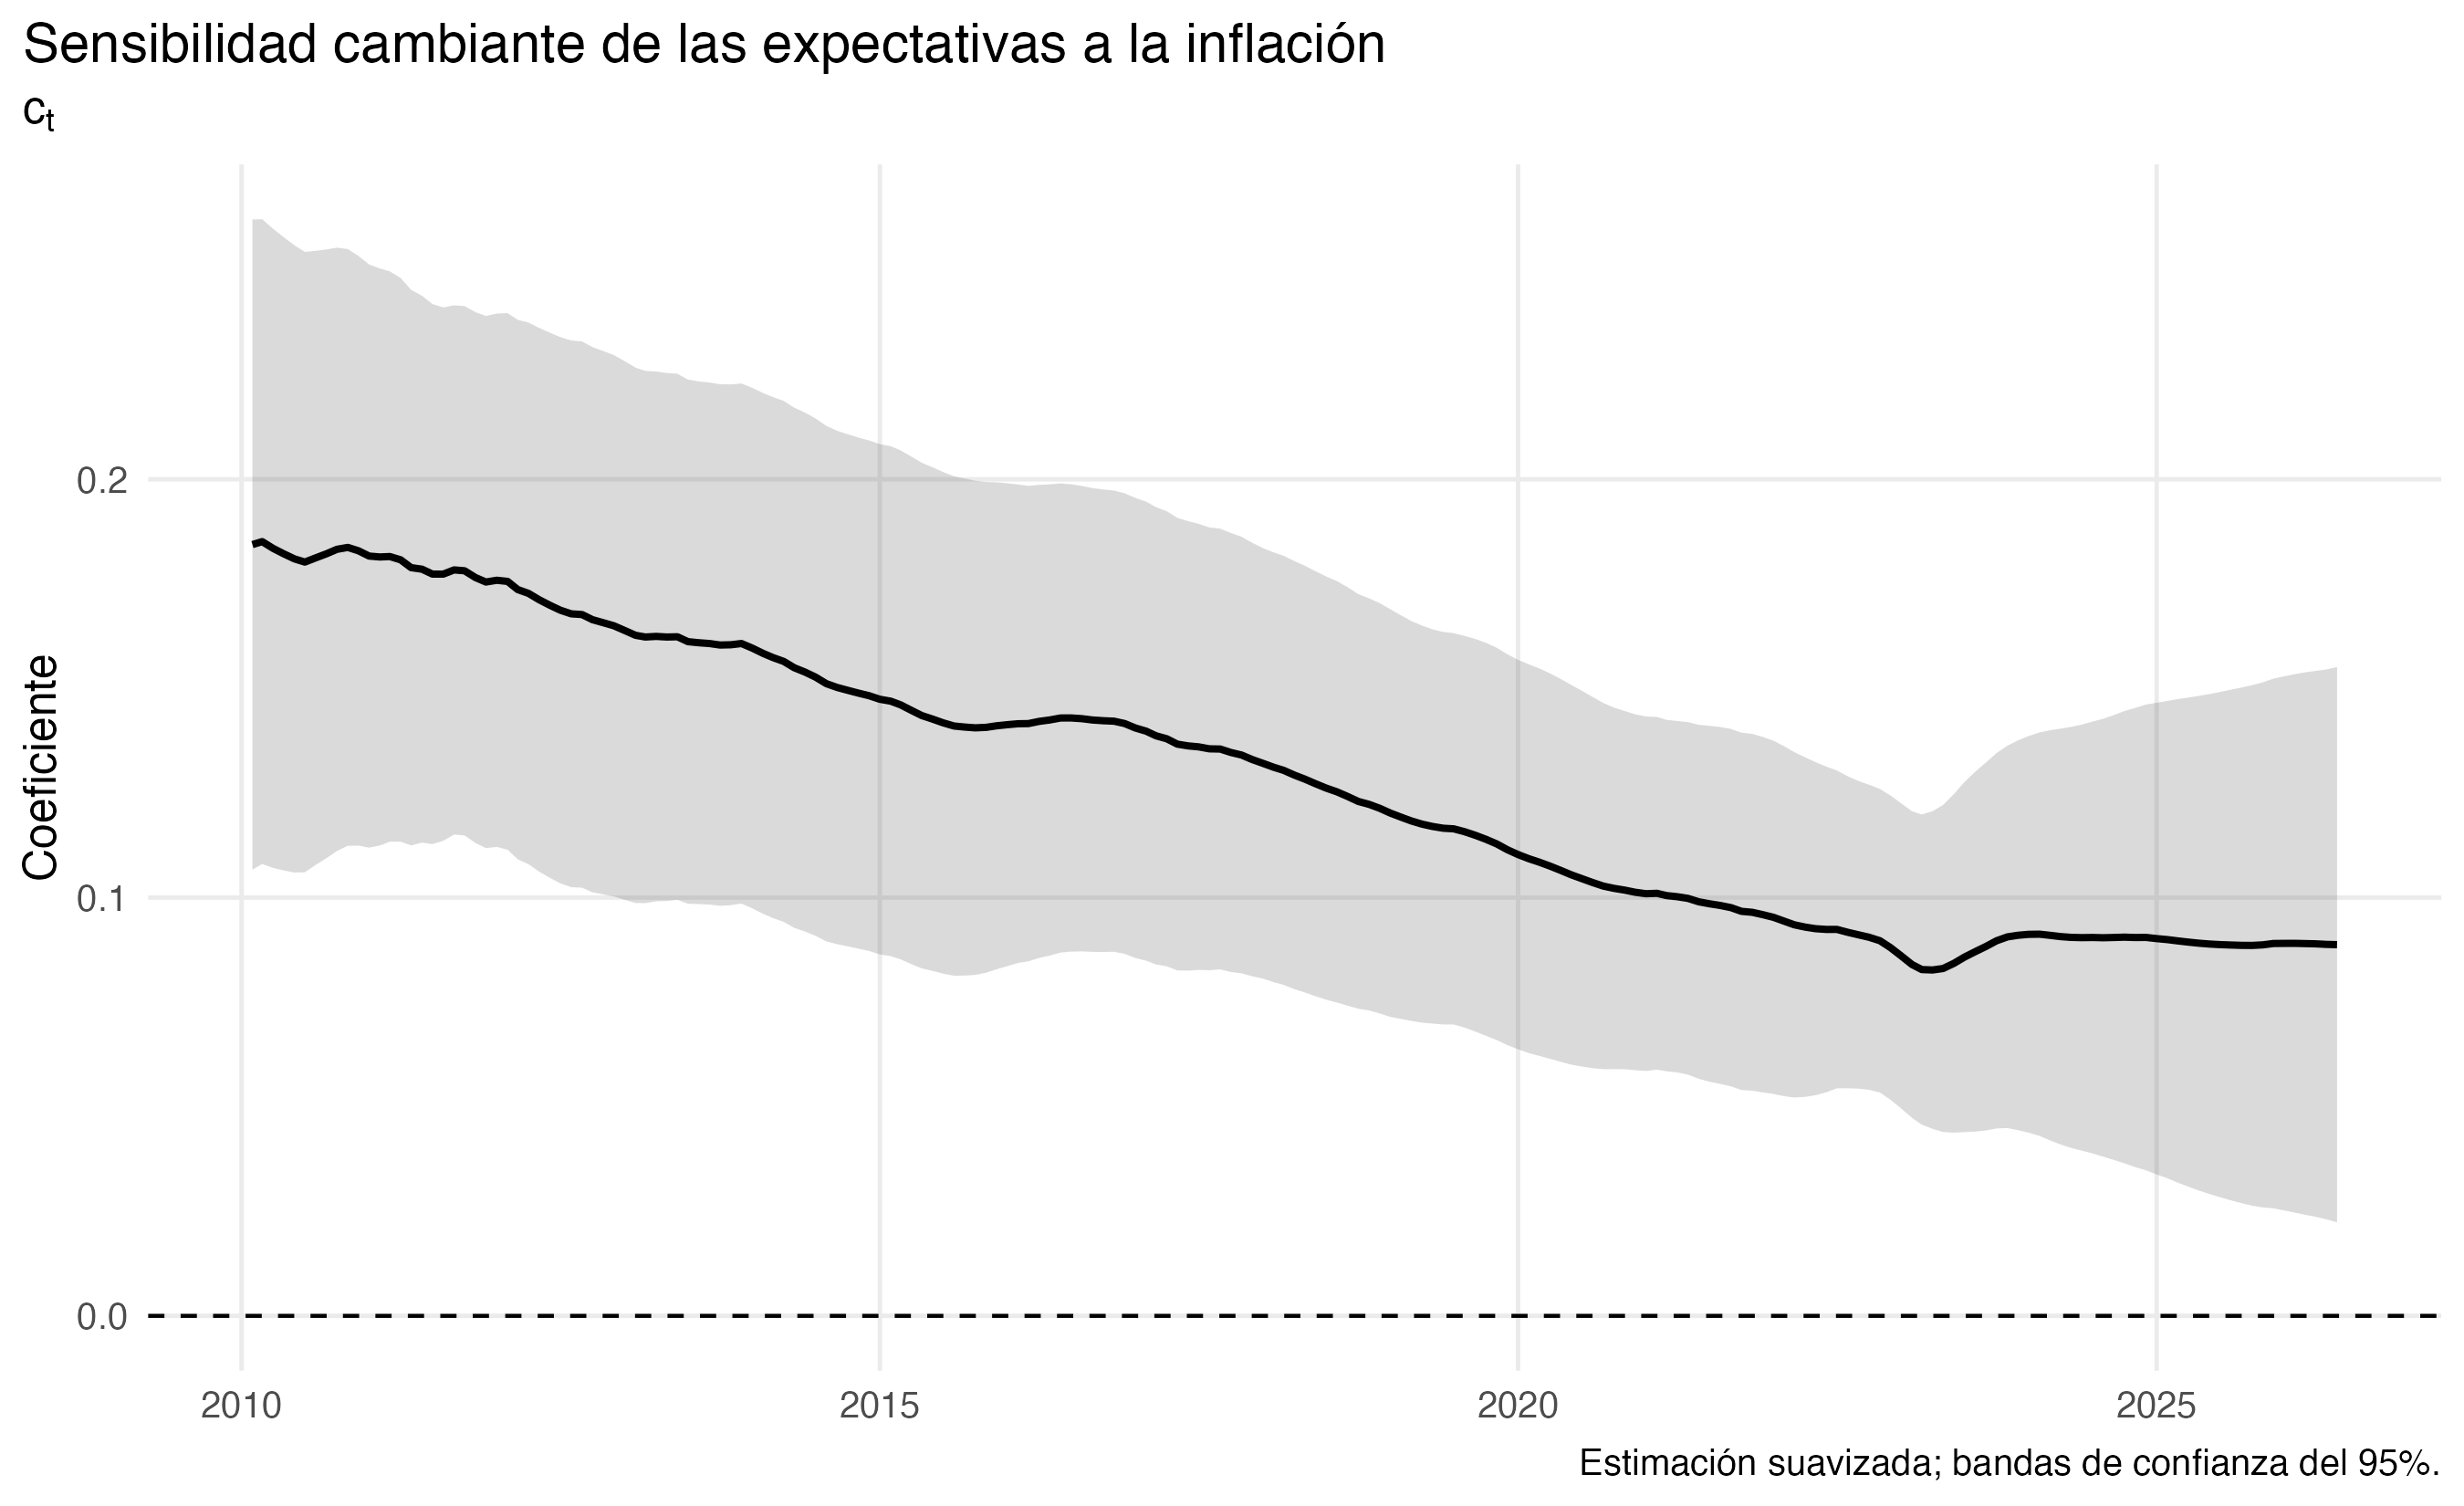
\includegraphics[width=1\linewidth,height=\textheight,keepaspectratio]{Data y resultados/resultados_objetivo2_TVP_VAR/figura_02_c_t.png}

}

\subcaption{\label{fig-parametros-tvp-2}Sensibilidad frente a la
inflación, \(c_t\)}

\end{minipage}%

\caption{\label{fig-parametros-tvp}Parámetros variantes de la ecuación
de expectativas}

\end{figure}%

\textbf{Nota.} Estimaciones suavizadas mediante filtro de Kalman. Las
bandas corresponden a intervalos de confianza aproximados del 95 \%.
Elaboración propia.

El resultado de mayor interés económico en la
Figura~\ref{fig-parametros-tvp} corresponde a la trayectoria de \(c_t\),
que recoge la sensibilidad cambiante de las expectativas a 24 meses
frente a la inflación observada rezagada. Una reducción de este
coeficiente implica que las variaciones de la inflación corriente tienen
una incidencia progresivamente menor sobre la formación de expectativas
de mediano plazo. La trayectoria estimada debe interpretarse, por tanto,
como evidencia del grado de desacoplamiento entre ambas variables y no
como una medida aislada de credibilidad. En términos generales, la
evolución de \(c_t\) debería contrastarse con la obtenida mediante las
regresiones móviles: la coincidencia en la dirección del cambio
constituye evidencia de consistencia entre dos aproximaciones
econométricas distintas.

Por su parte, \(c_{0t}\) muestra cambios en el componente autónomo de la
ecuación de expectativas. Este parámetro no constituye por sí mismo el
ancla de inflación de largo plazo; su interpretación económica surge al
combinarlo con \(c_t\) y con la persistencia de las expectativas, \(d\),
en la expresión de equilibrio utilizada para obtener \(\pi_t^*\). En
consecuencia, la lectura conjunta de ambos parámetros resulta más
informativa que la interpretación aislada de sus niveles.

\subsection{Proxy dinámica de credibilidad y grado de
anclaje}\label{proxy-dinuxe1mica-de-credibilidad-y-grado-de-anclaje}

\begin{figure}

\centering{

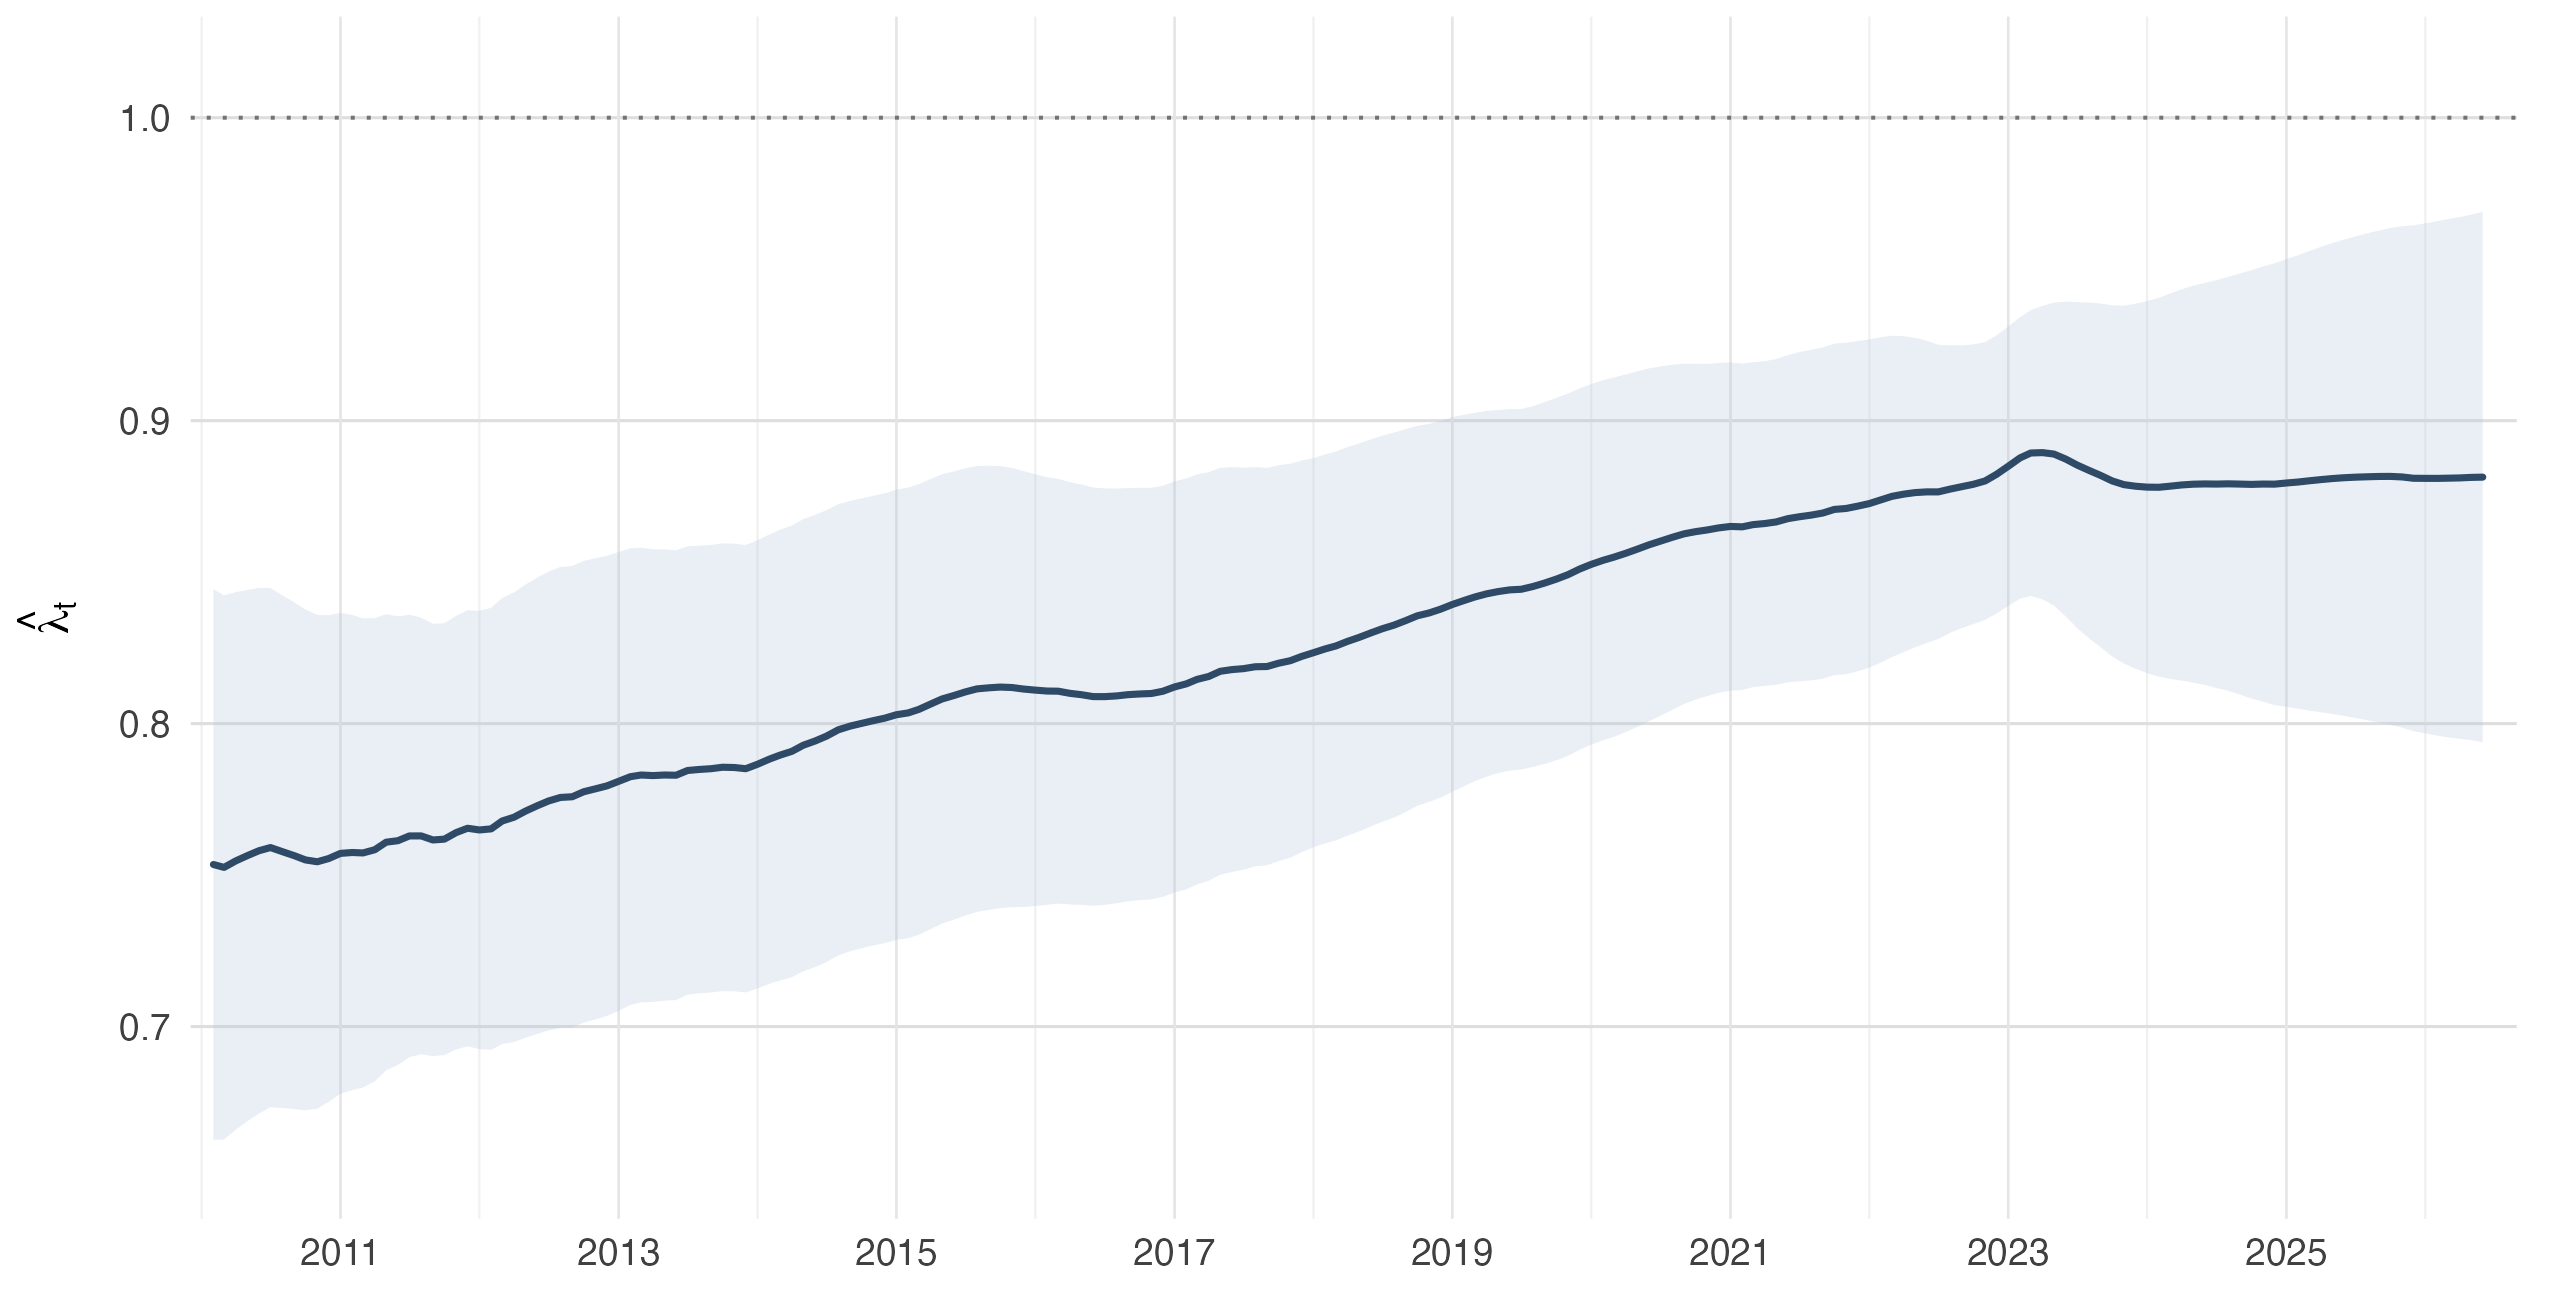
\includegraphics[width=0.92\linewidth,height=\textheight,keepaspectratio]{Data y resultados/resultados_objetivo2_TVP_VAR/figura_03_lambda_t.png}

}

\caption{\label{fig-lambda-tvp}Evolución de la proxy dinámica de
credibilidad}

\end{figure}%

\textbf{Nota.} La línea representa la estimación suavizada de
\(\lambda_t=1-c_t/(1-d)\) y el área sombreada su intervalo de confianza
aproximado del 95 \%. Valores más próximos a uno indican un mayor
desacoplamiento de las expectativas respecto de la inflación observada.
Elaboración propia.

La Figura~\ref{fig-lambda-tvp} muestra una trayectoria creciente de la
proxy de credibilidad a lo largo de la muestra. El valor estimado pasa
de aproximadamente 0.753 al inicio del período a 0.881 al final,
mientras que su promedio se sitúa en 0.829. Más que un cambio abrupto,
la dinámica evidencia un proceso gradual de fortalecimiento: las
expectativas a 24 meses se vuelven progresivamente menos dependientes de
la inflación observada. Este patrón es consistente con la interpretación
de Maria Demertzis (2009), según la cual una mayor separación entre la
dinámica de inflación y la de las expectativas constituye evidencia de
mayor credibilidad del ancla nominal.

Desde una perspectiva temporal, el fortalecimiento es particularmente
relevante porque la proxy no muestra un deterioro persistente durante el
episodio inflacionario más reciente. Aun cuando la inflación observada
se alejó temporalmente de la meta, \(\lambda_t\) permaneció en niveles
elevados y posteriormente mostró solo una corrección moderada. Esto
sugiere que el aumento de la inflación no se trasladó en igual magnitud
a la formación de expectativas de mediano plazo. En el lenguaje de
(\textbf{strohsal\_melnick\_nautz2015?}), este comportamiento es más
consistente con un anclaje que puede experimentar fluctuaciones
transitorias sin necesariamente transformarse en un proceso persistente
de desanclaje.

En conjunto, la trayectoria de \(\lambda_t\) refuerza la evidencia
obtenida mediante las regresiones móviles. Mientras estas últimas
muestran cómo la sensibilidad estimada cambia entre ventanas sucesivas,
el modelo TVP--VAR permite representar el mismo fenómeno mediante una
evolución continua de los parámetros. La coincidencia cualitativa de
ambas aproximaciones constituye evidencia favorable a la hipótesis de un
fortalecimiento gradual del anclaje durante el período analizado.

\subsection{Evolución del ancla inflacionaria
implícita}\label{evoluciuxf3n-del-ancla-inflacionaria-impluxedcita}

\begin{figure}

\centering{

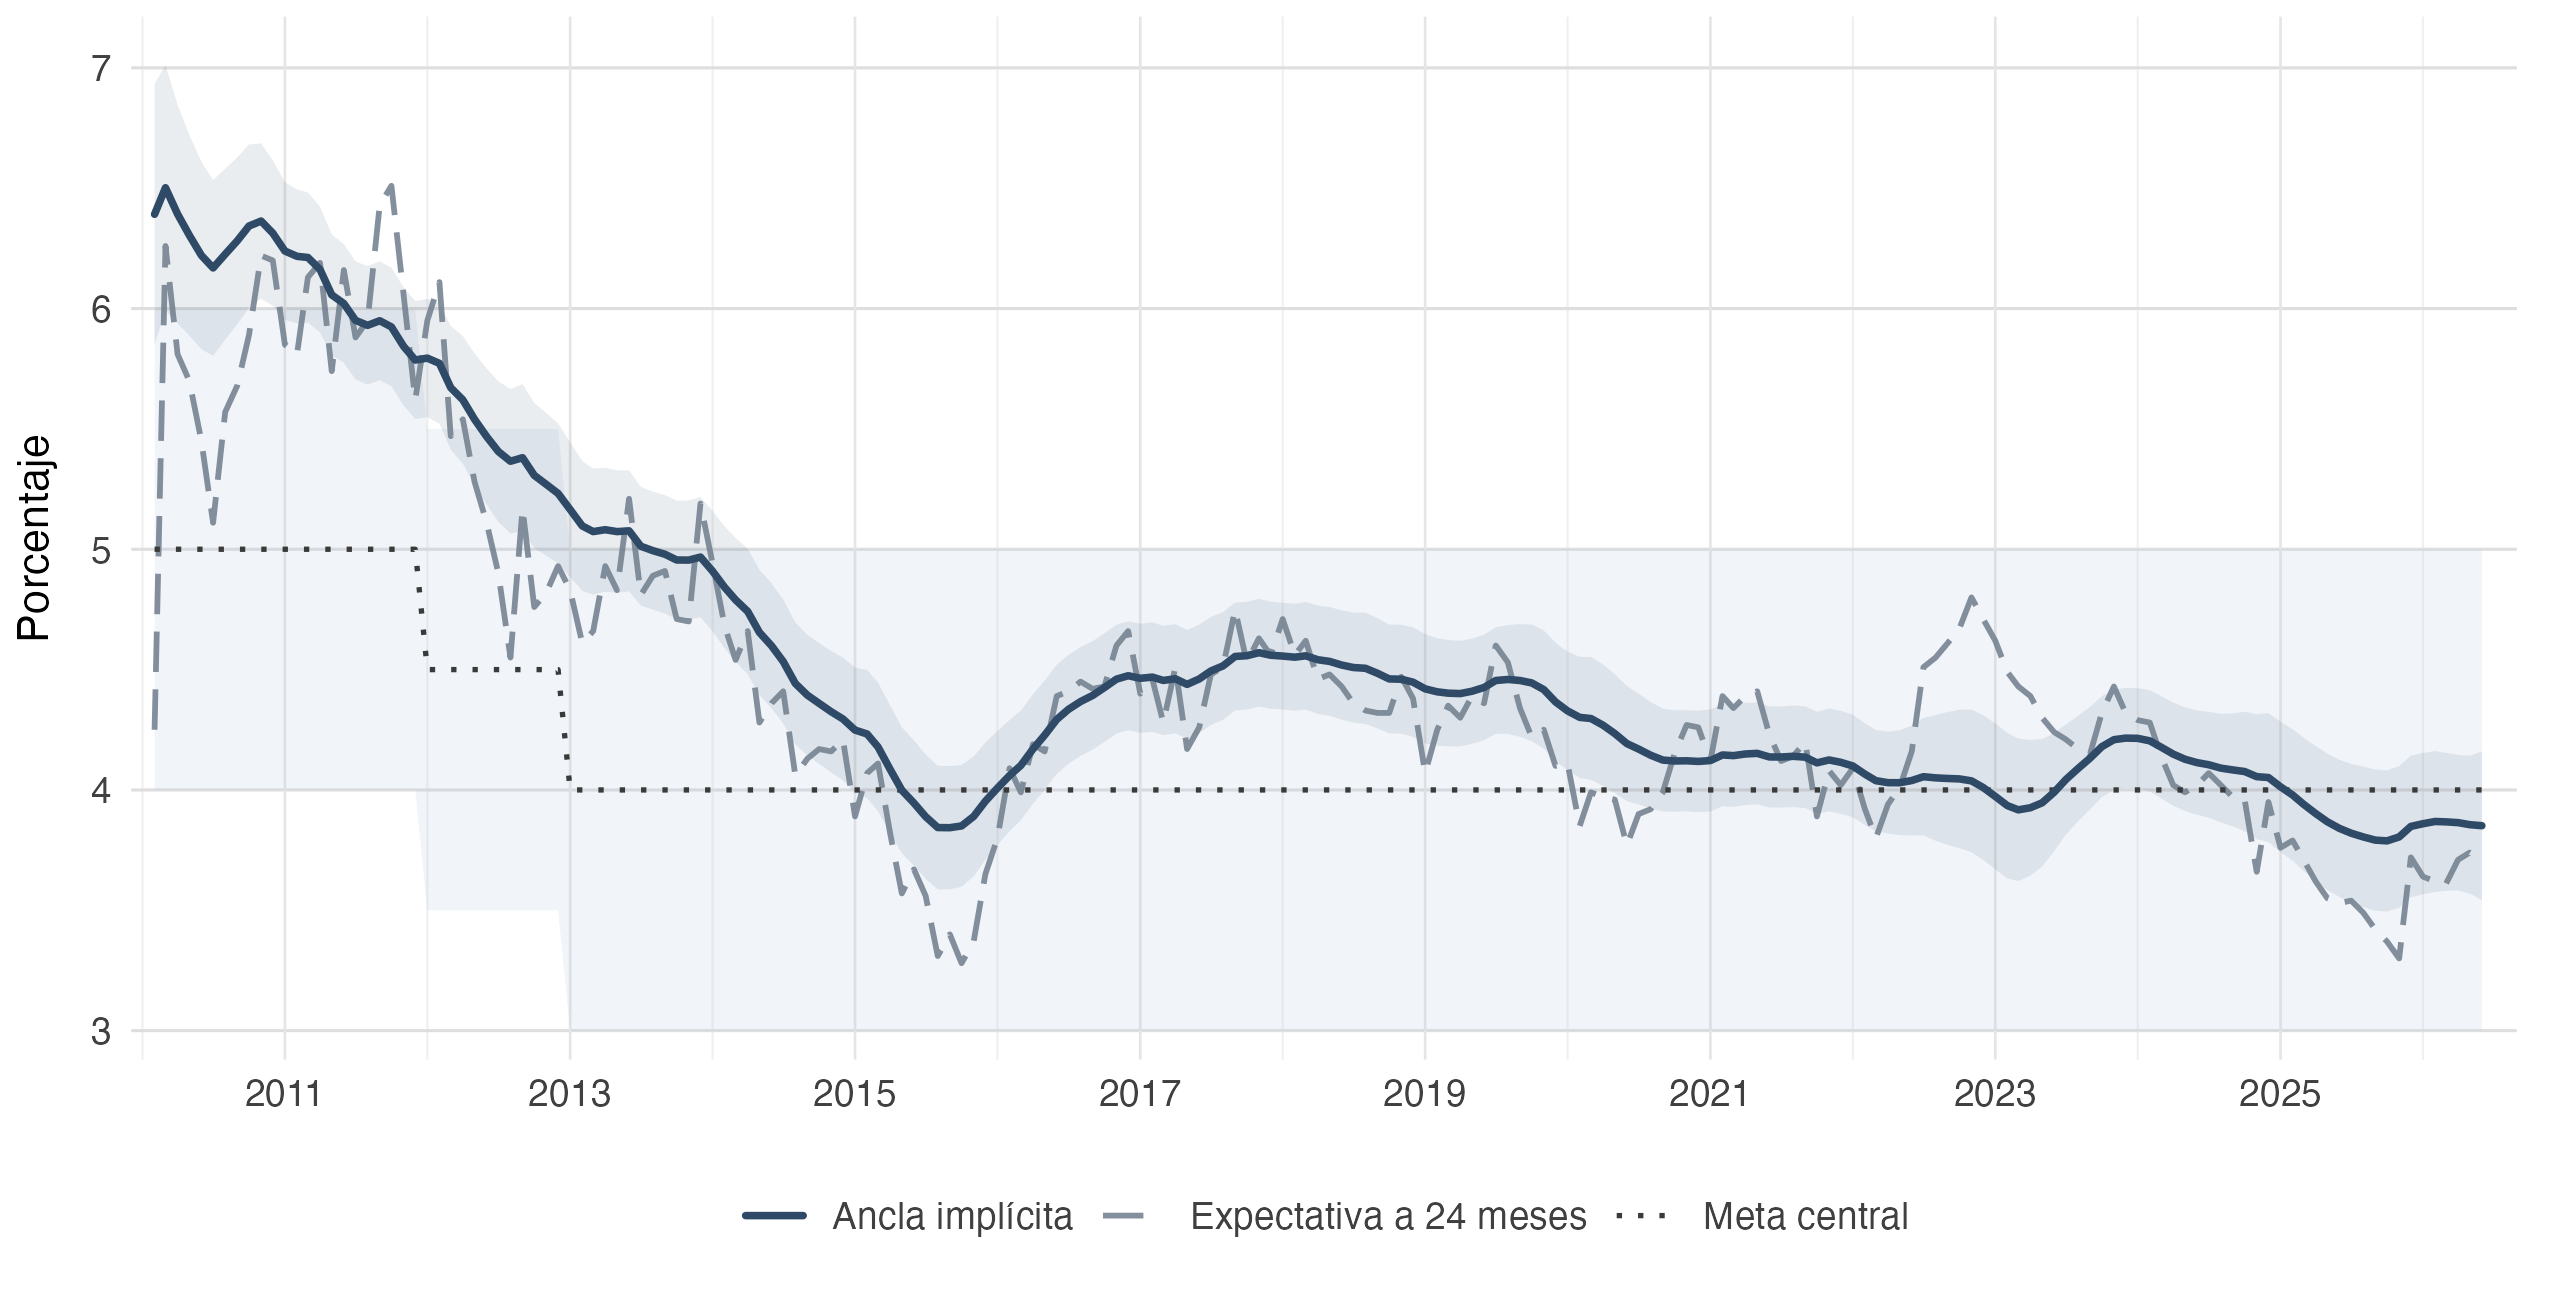
\includegraphics[width=0.92\linewidth,height=\textheight,keepaspectratio]{Data y resultados/resultados_objetivo2_TVP_VAR/figura_04_ancla_implicita.png}

}

\caption{\label{fig-ancla-implicita}Ancla inflacionaria implícita y
expectativas de inflación a 24 meses}

\end{figure}%

\textbf{Nota.} El ancla implícita \(\pi_t^*\) se obtiene a partir de los
parámetros estimados del TVP--VAR y no impone la meta oficial en su
construcción. El área sombreada representa el rango de tolerancia
alrededor de la meta central vigente. Elaboración propia.

La proxy \(\lambda_t\) indica cuánto se desacoplan las expectativas de
la inflación pasada, pero no identifica por sí misma el nivel alrededor
del cual se encuentran ancladas. Para ello, el modelo permite recuperar
\(\pi_t^*\), es decir, el valor de inflación implícito en la relación de
equilibrio entre inflación y expectativas. Esta distinción es central:
un régimen de mayor credibilidad no solo debería mostrar una elevada
separación respecto de fluctuaciones transitorias de inflación, sino
también un ancla implícita compatible con el objetivo anunciado por la
autoridad monetaria.

Los resultados muestran que el ancla implícita se aproxima
progresivamente al objetivo de política monetaria. En promedio,
\(\pi_t^*\) se ubica en 4.57 \%, pero la trayectoria es más informativa
que ese promedio: parte de aproximadamente 6.39 \% y finaliza en 3.85
\%. Asimismo, el error absoluto medio respecto de la meta es de 0.46
puntos porcentuales y el ancla permanece dentro del rango meta en
aproximadamente 85.3 \% de los meses. En consecuencia, la evidencia no
solo muestra un aumento de \(\lambda_t\), sino también una convergencia
del nivel implícito de largo plazo hacia valores compatibles con el
objetivo anunciado.

El comportamiento durante el episodio inflacionario de 2021--2023
resulta particularmente informativo. Aunque la inflación observada se
alejó de la meta, el ancla implícita permaneció comparativamente estable
y próxima al objetivo central. Esta divergencia sugiere que los agentes
no incorporaron de manera permanente toda la perturbación inflacionaria
reciente en su valoración del nivel de inflación de mediano plazo.
Interpretado conjuntamente con la elevada trayectoria de \(\lambda_t\),
el resultado es compatible con expectativas que permanecieron
relativamente ancladas pese a un choque inflacionario de magnitud
considerable.

\subsection{Robustez y limitaciones de la
especificación}\label{robustez-y-limitaciones-de-la-especificaciuxf3n}

El principal diagnóstico que requiere cautela es la autocorrelación de
los residuos de la ecuación de inflación cuando se utiliza la variación
interanual del IPC. La incorporación de rezagos adicionales no elimina
completamente este patrón, lo que sugiere que parte de la persistencia
residual puede estar asociada a la propia construcción solapada de la
tasa interanual. Por esta razón, la inflación interanual se mantiene
como especificación principal por su correspondencia de escala con las
expectativas expresadas en términos anuales, pero se complementa con
medidas alternativas de inflación como ejercicio de robustez.

\begin{longtable}[]{@{}
  >{\raggedright\arraybackslash}p{(\linewidth - 8\tabcolsep) * \real{0.1765}}
  >{\centering\arraybackslash}p{(\linewidth - 8\tabcolsep) * \real{0.2706}}
  >{\centering\arraybackslash}p{(\linewidth - 8\tabcolsep) * \real{0.1765}}
  >{\centering\arraybackslash}p{(\linewidth - 8\tabcolsep) * \real{0.2353}}
  >{\centering\arraybackslash}p{(\linewidth - 8\tabcolsep) * \real{0.1412}}@{}}

\caption{\label{tbl-robustez-msaa}Robustez de la proxy de credibilidad
ante medidas alternativas de inflación}

\tabularnewline

\toprule\noalign{}
\begin{minipage}[b]{\linewidth}\raggedright
Especificación
\end{minipage} & \begin{minipage}[b]{\linewidth}\centering
Correlación de lambda
\end{minipage} & \begin{minipage}[b]{\linewidth}\centering
MAE de lambda
\end{minipage} & \begin{minipage}[b]{\linewidth}\centering
Correlación de pi*
\end{minipage} & \begin{minipage}[b]{\linewidth}\centering
MAE de pi*
\end{minipage} \\
\midrule\noalign{}
\endhead
\bottomrule\noalign{}
\endlastfoot
YOYIPC & 1.000 & 0.007 & 1.000 & 0.023 \\
MSAA & 0.983 & 0.022 & 0.826 & 0.338 \\

\end{longtable}

La robustez con inflación mensual desestacionalizada anualizada es
especialmente relevante. Bajo esta transformación desaparece la
evidencia de autocorrelación residual en la ecuación de inflación,
mientras que la trayectoria de \(\lambda_t\) conserva una correlación
cercana a 0.98 con la especificación base y una diferencia absoluta
media reducida. La estabilidad de la proxy frente a una medida sin el
solapamiento de doce meses indica que la conclusión sobre el
fortalecimiento del anclaje no depende exclusivamente de la persistencia
mecánica de la inflación interanual. El ancla implícita presenta una
sensibilidad algo mayor a la medida de inflación empleada, por lo que
sus niveles deben interpretarse con mayor cautela que la trayectoria de
\(\lambda_t\).

\subsection{Síntesis de los resultados del
TVP--VAR}\label{suxedntesis-de-los-resultados-del-tvpvar}

En síntesis, el TVP--VAR restringido aporta dos resultados
complementarios sobre el anclaje de las expectativas de inflación en
Guatemala. Primero, la proxy dinámica de credibilidad muestra un aumento
gradual del desacoplamiento entre las expectativas a 24 meses y la
inflación observada, reforzando la evidencia obtenida mediante las
regresiones móviles. Segundo, el ancla inflacionaria implícita converge
hacia valores próximos a la meta oficial y permanece relativamente
estable incluso durante el episodio inflacionario reciente. Considerados
conjuntamente, ambos resultados son compatibles con un proceso gradual
de fortalecimiento del anclaje de las expectativas de mediano plazo
durante el período de análisis.

La persistencia de autocorrelación en la ecuación auxiliar de inflación
interanual constituye una limitación de la especificación base; sin
embargo, los ejercicios con medidas alternativas muestran que la
trayectoria principal de \(\lambda_t\) se mantiene cuando se elimina el
componente de solapamiento de la inflación interanual. La evidencia
obtenida en esta sección caracteriza el grado y la evolución del
anclaje; el siguiente bloque del análisis amplía esta perspectiva al
examinar cómo responden las expectativas ante choques macroeconómicos
identificados dentro de un marco VAR.

\phantomsection\label{refs}
\begin{CSLReferences}{1}{0}
\bibitem[\citeproctext]{ref-demertzis_marcellino_viegi2012}
Maria Demertzis, Nicola Viegi, Massimiliano Marcellino. 2009. {«A
Credibility Proxy: Tracking US Monetary Developments»}. \emph{The BE
Journal of Macroeconomics} 12 (1).

\end{CSLReferences}




\end{document}
